\documentclass{article}
\usepackage{graphicx} % Required for inserting images
\usepackage{amsmath}
\usepackage{geometry}
\usepackage{amssymb}
\usepackage{color}
\usepackage{CJKutf8}
\usepackage{float}
\usepackage{subfigure}
\usepackage{listings}
\usepackage{placeins}
\usepackage{enumitem}
\usepackage{booktabs}

\geometry{a4paper, scale=0.8}   
\linespread{2}
\definecolor{dark_green}{RGB}{0,102,51}
\title{Lab4 - IP}
\author{Jiaxi Zhang}
\date{\today}
\begin{document}
\maketitle
\begin{CJK*}{UTF8}{gbsn}

\section{A look at the captured trace}
\begin{figure}[H]
    \centering
    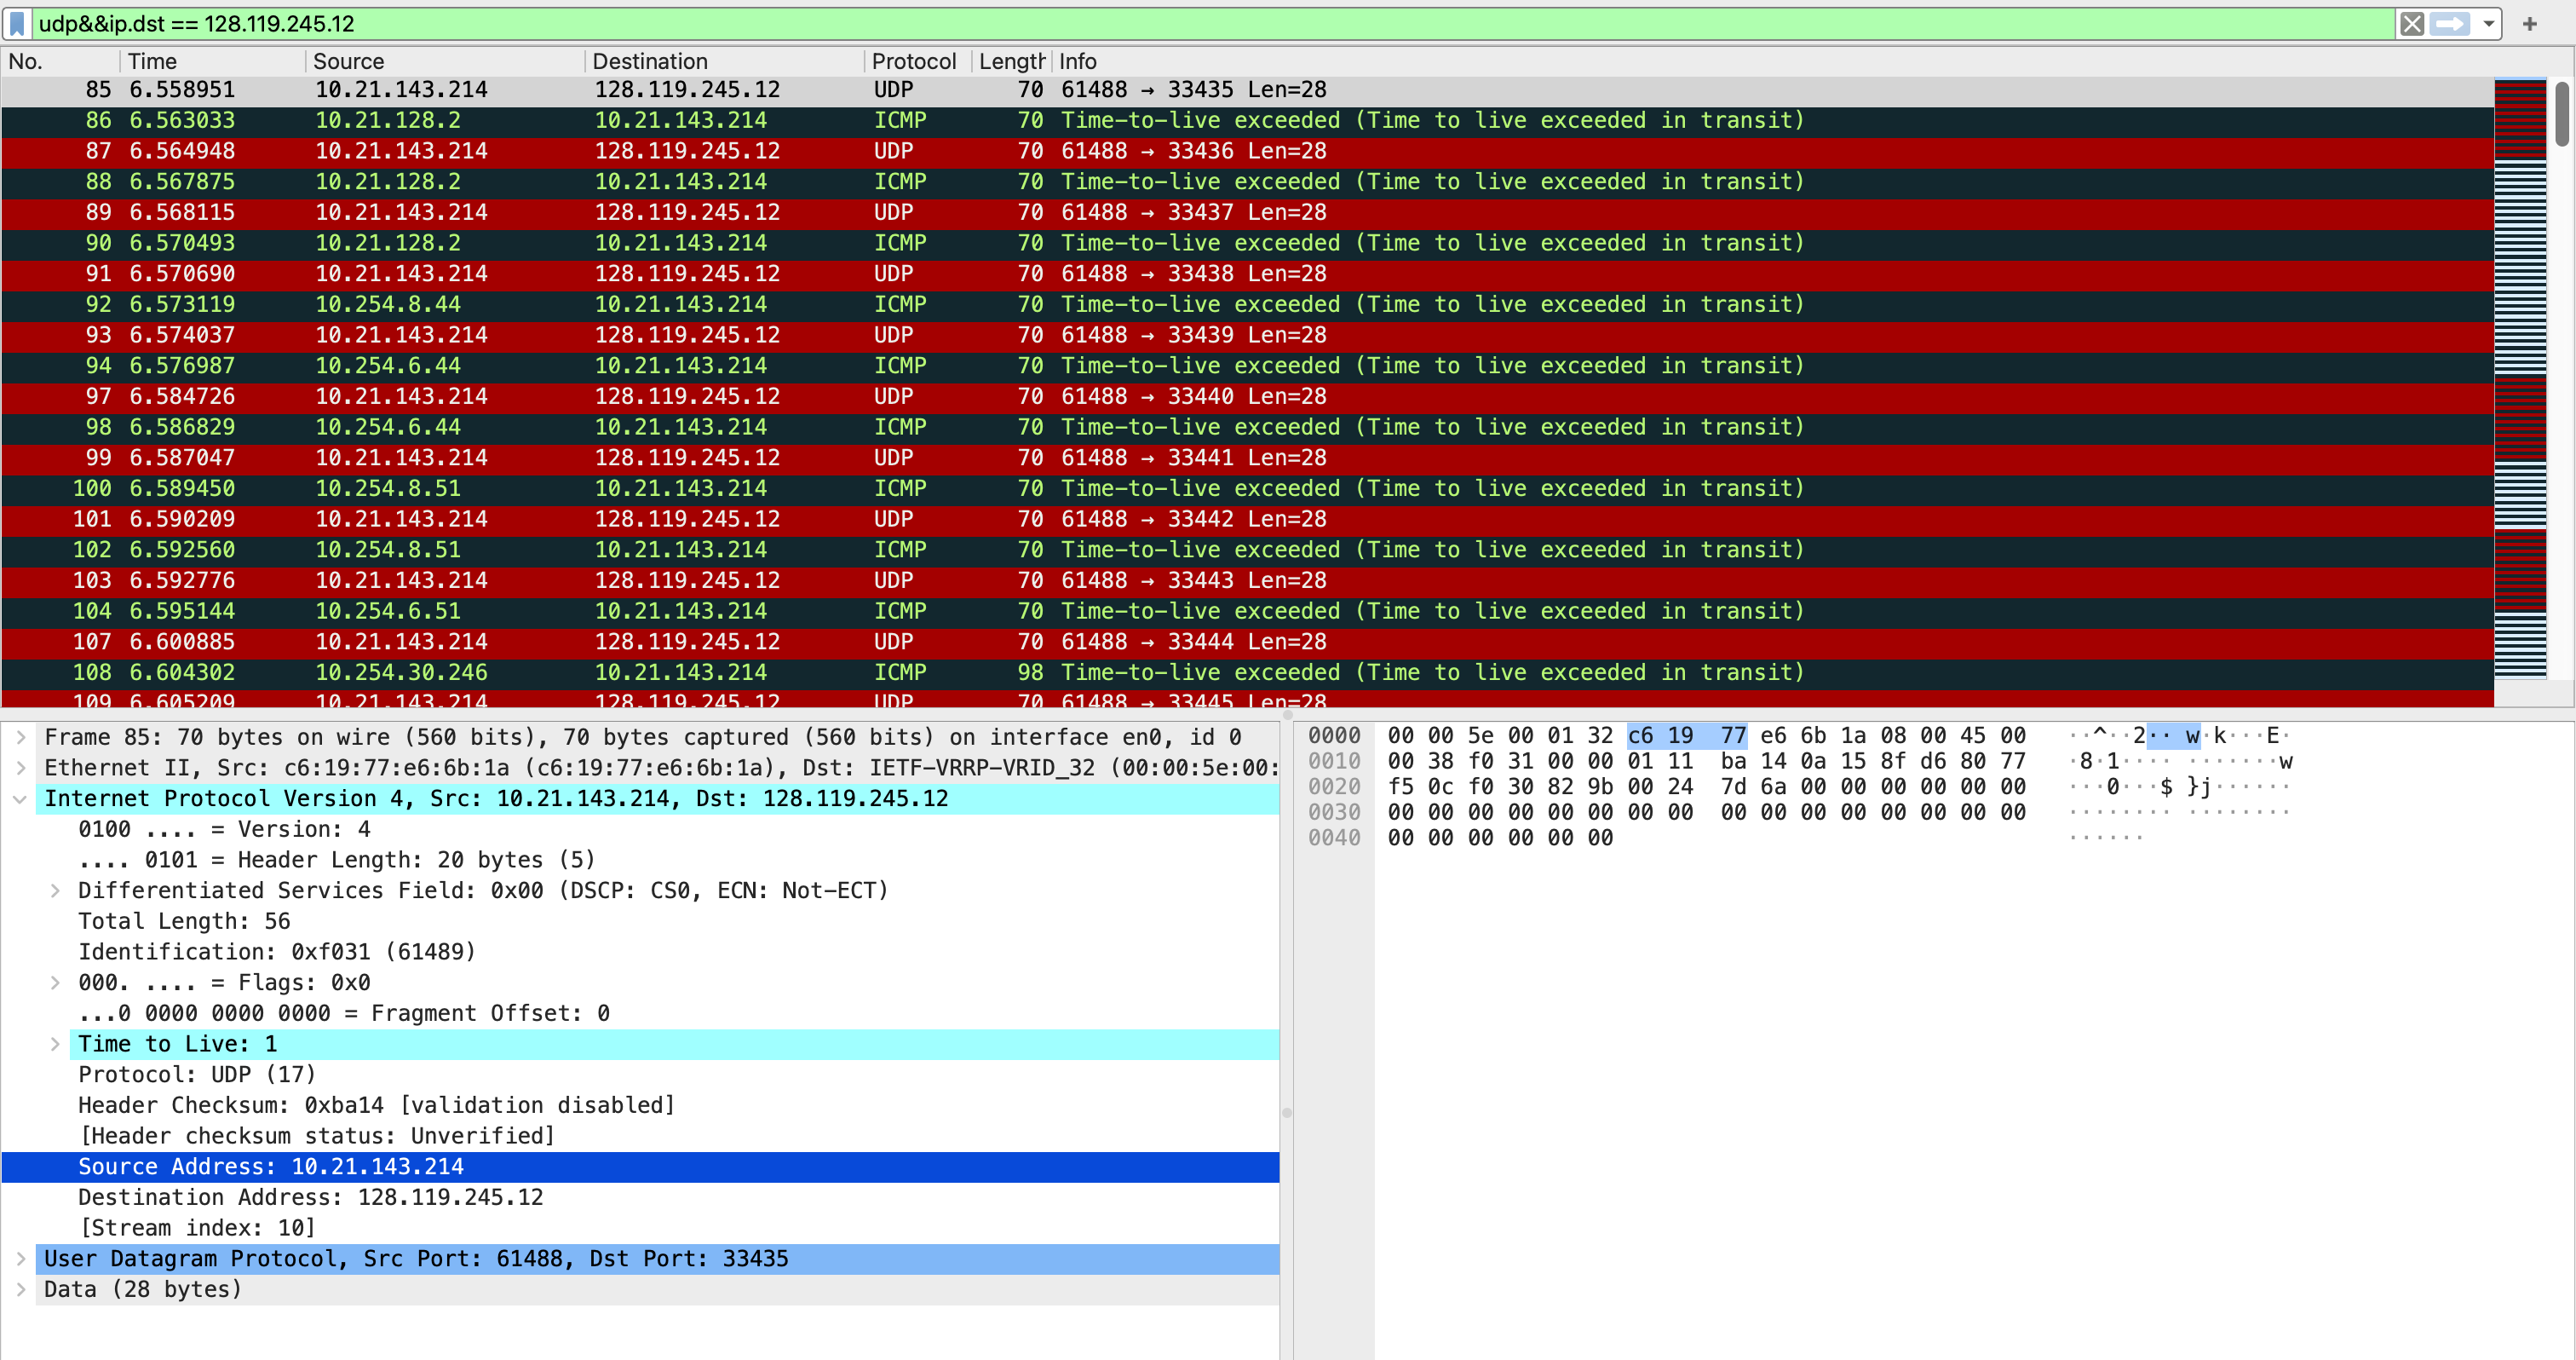
\includegraphics[width=1.0\textwidth]{0.png}
\end{figure}
\begin{figure}[H]
    \centering
    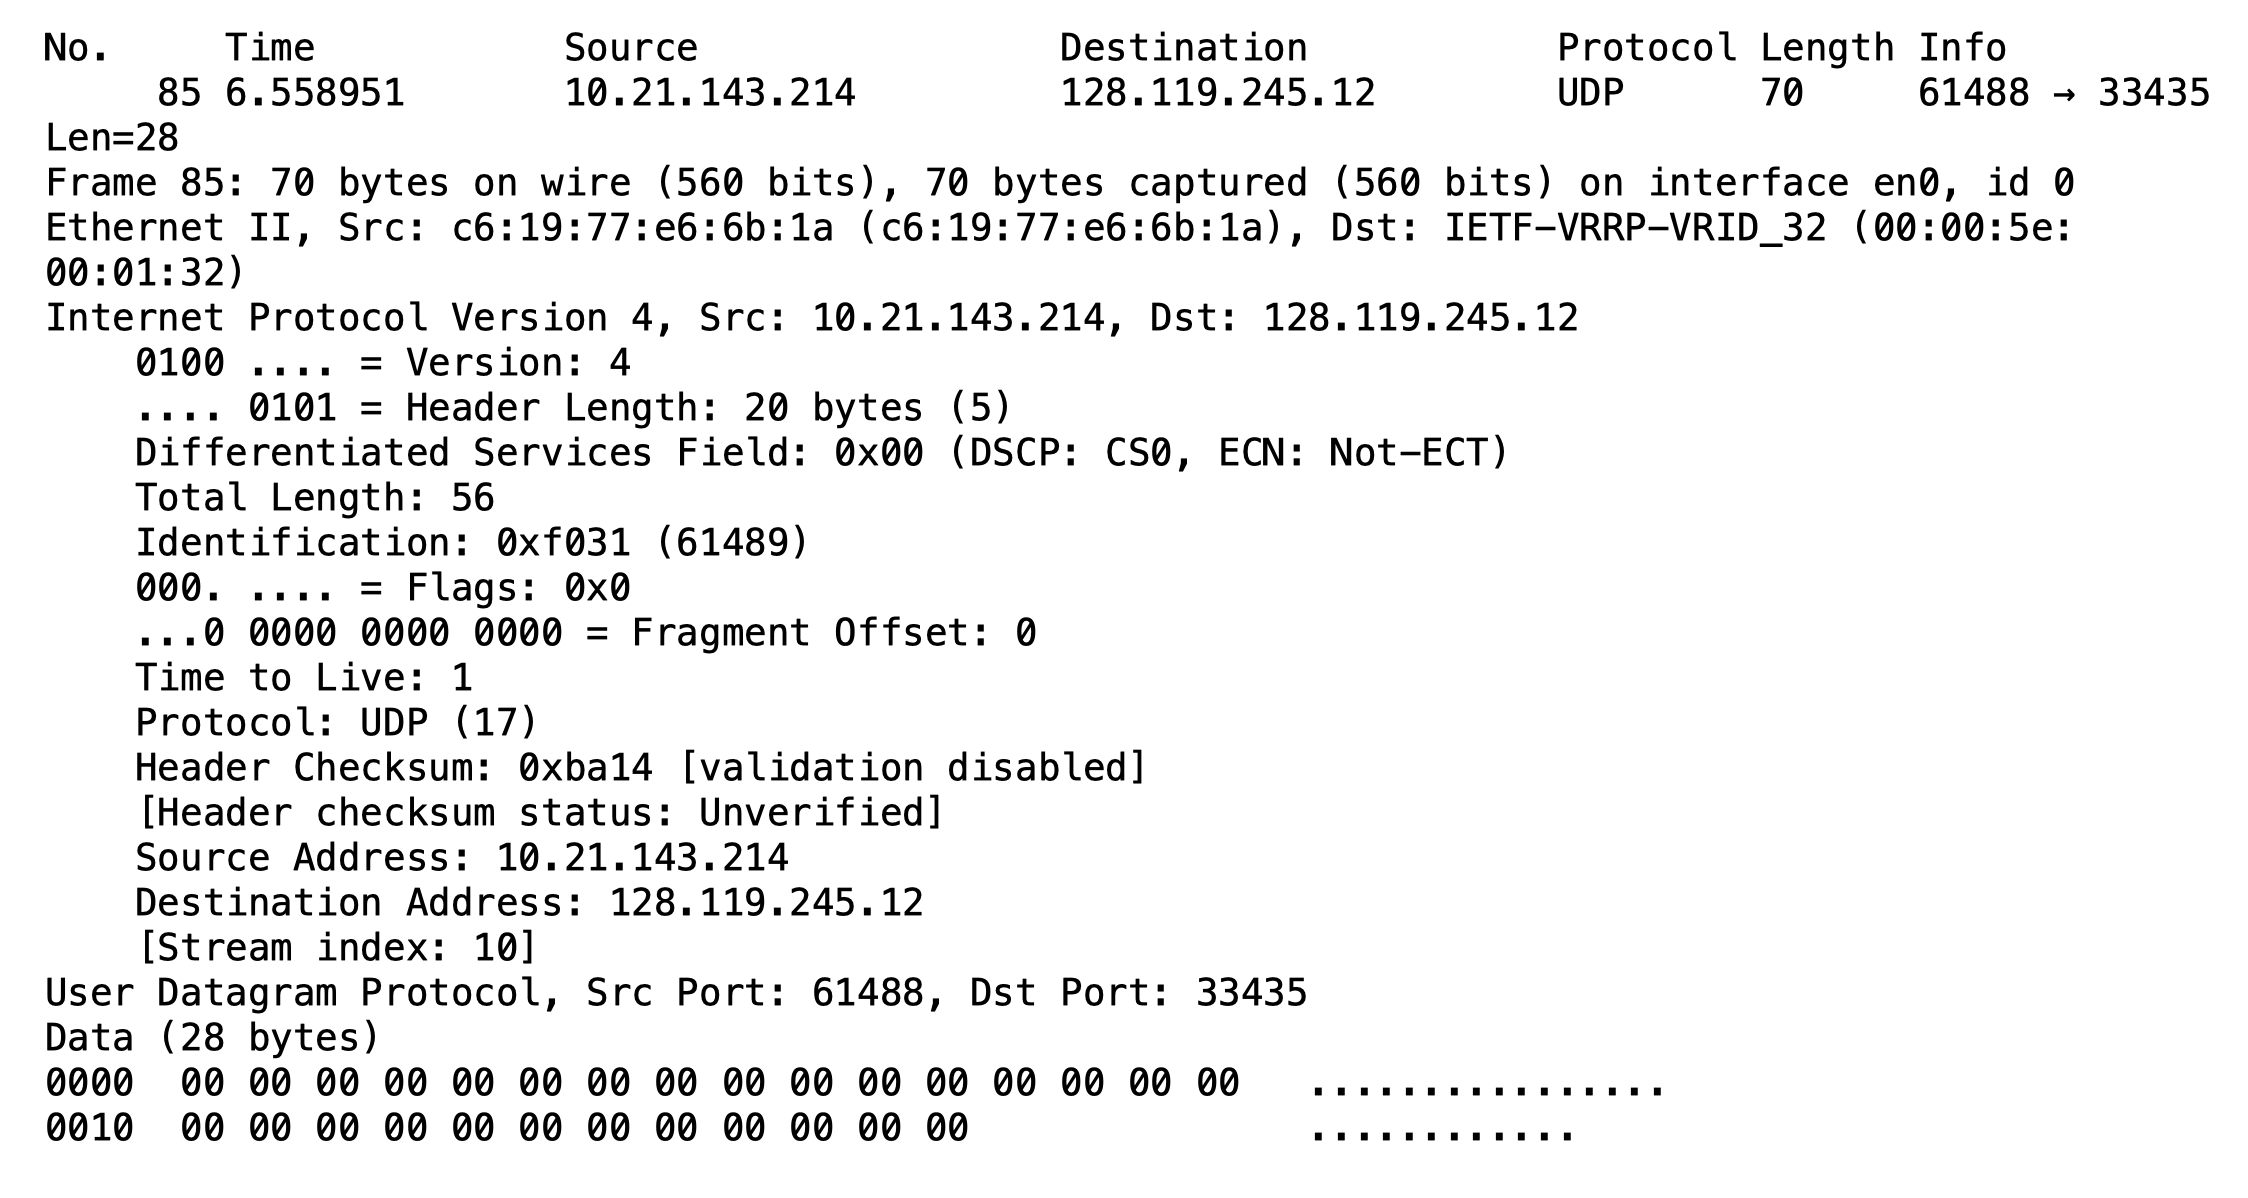
\includegraphics[width=1.0\textwidth]{0-1.png}
\end{figure}
The following questions are answered based on the above two figures.
\subsection{Question 1}
My IP address is 10.21.143.214
\subsection{Question 2}
The upper protocol is UDP, the protocol number is 17.
\subsection{Question 3}
IP header length is 20 bytes, the total length is 56 bytes.
Thus, the payload length is 56 - 20 = 36 bytes.
\subsection{Question 4}
This IP datagram is not fragmented. It can be seen from the screenshot that Fragment Offset is 0, and "Flags: 0x0" indicates that the datagram is not fragmented.
\section{Sorted by source port}
This is a screenshot after sorting by source port (with the arrow pointing down). It seems that since the arrow is pointing down, the time is in descending order.
\begin{figure}[H]
    \centering
    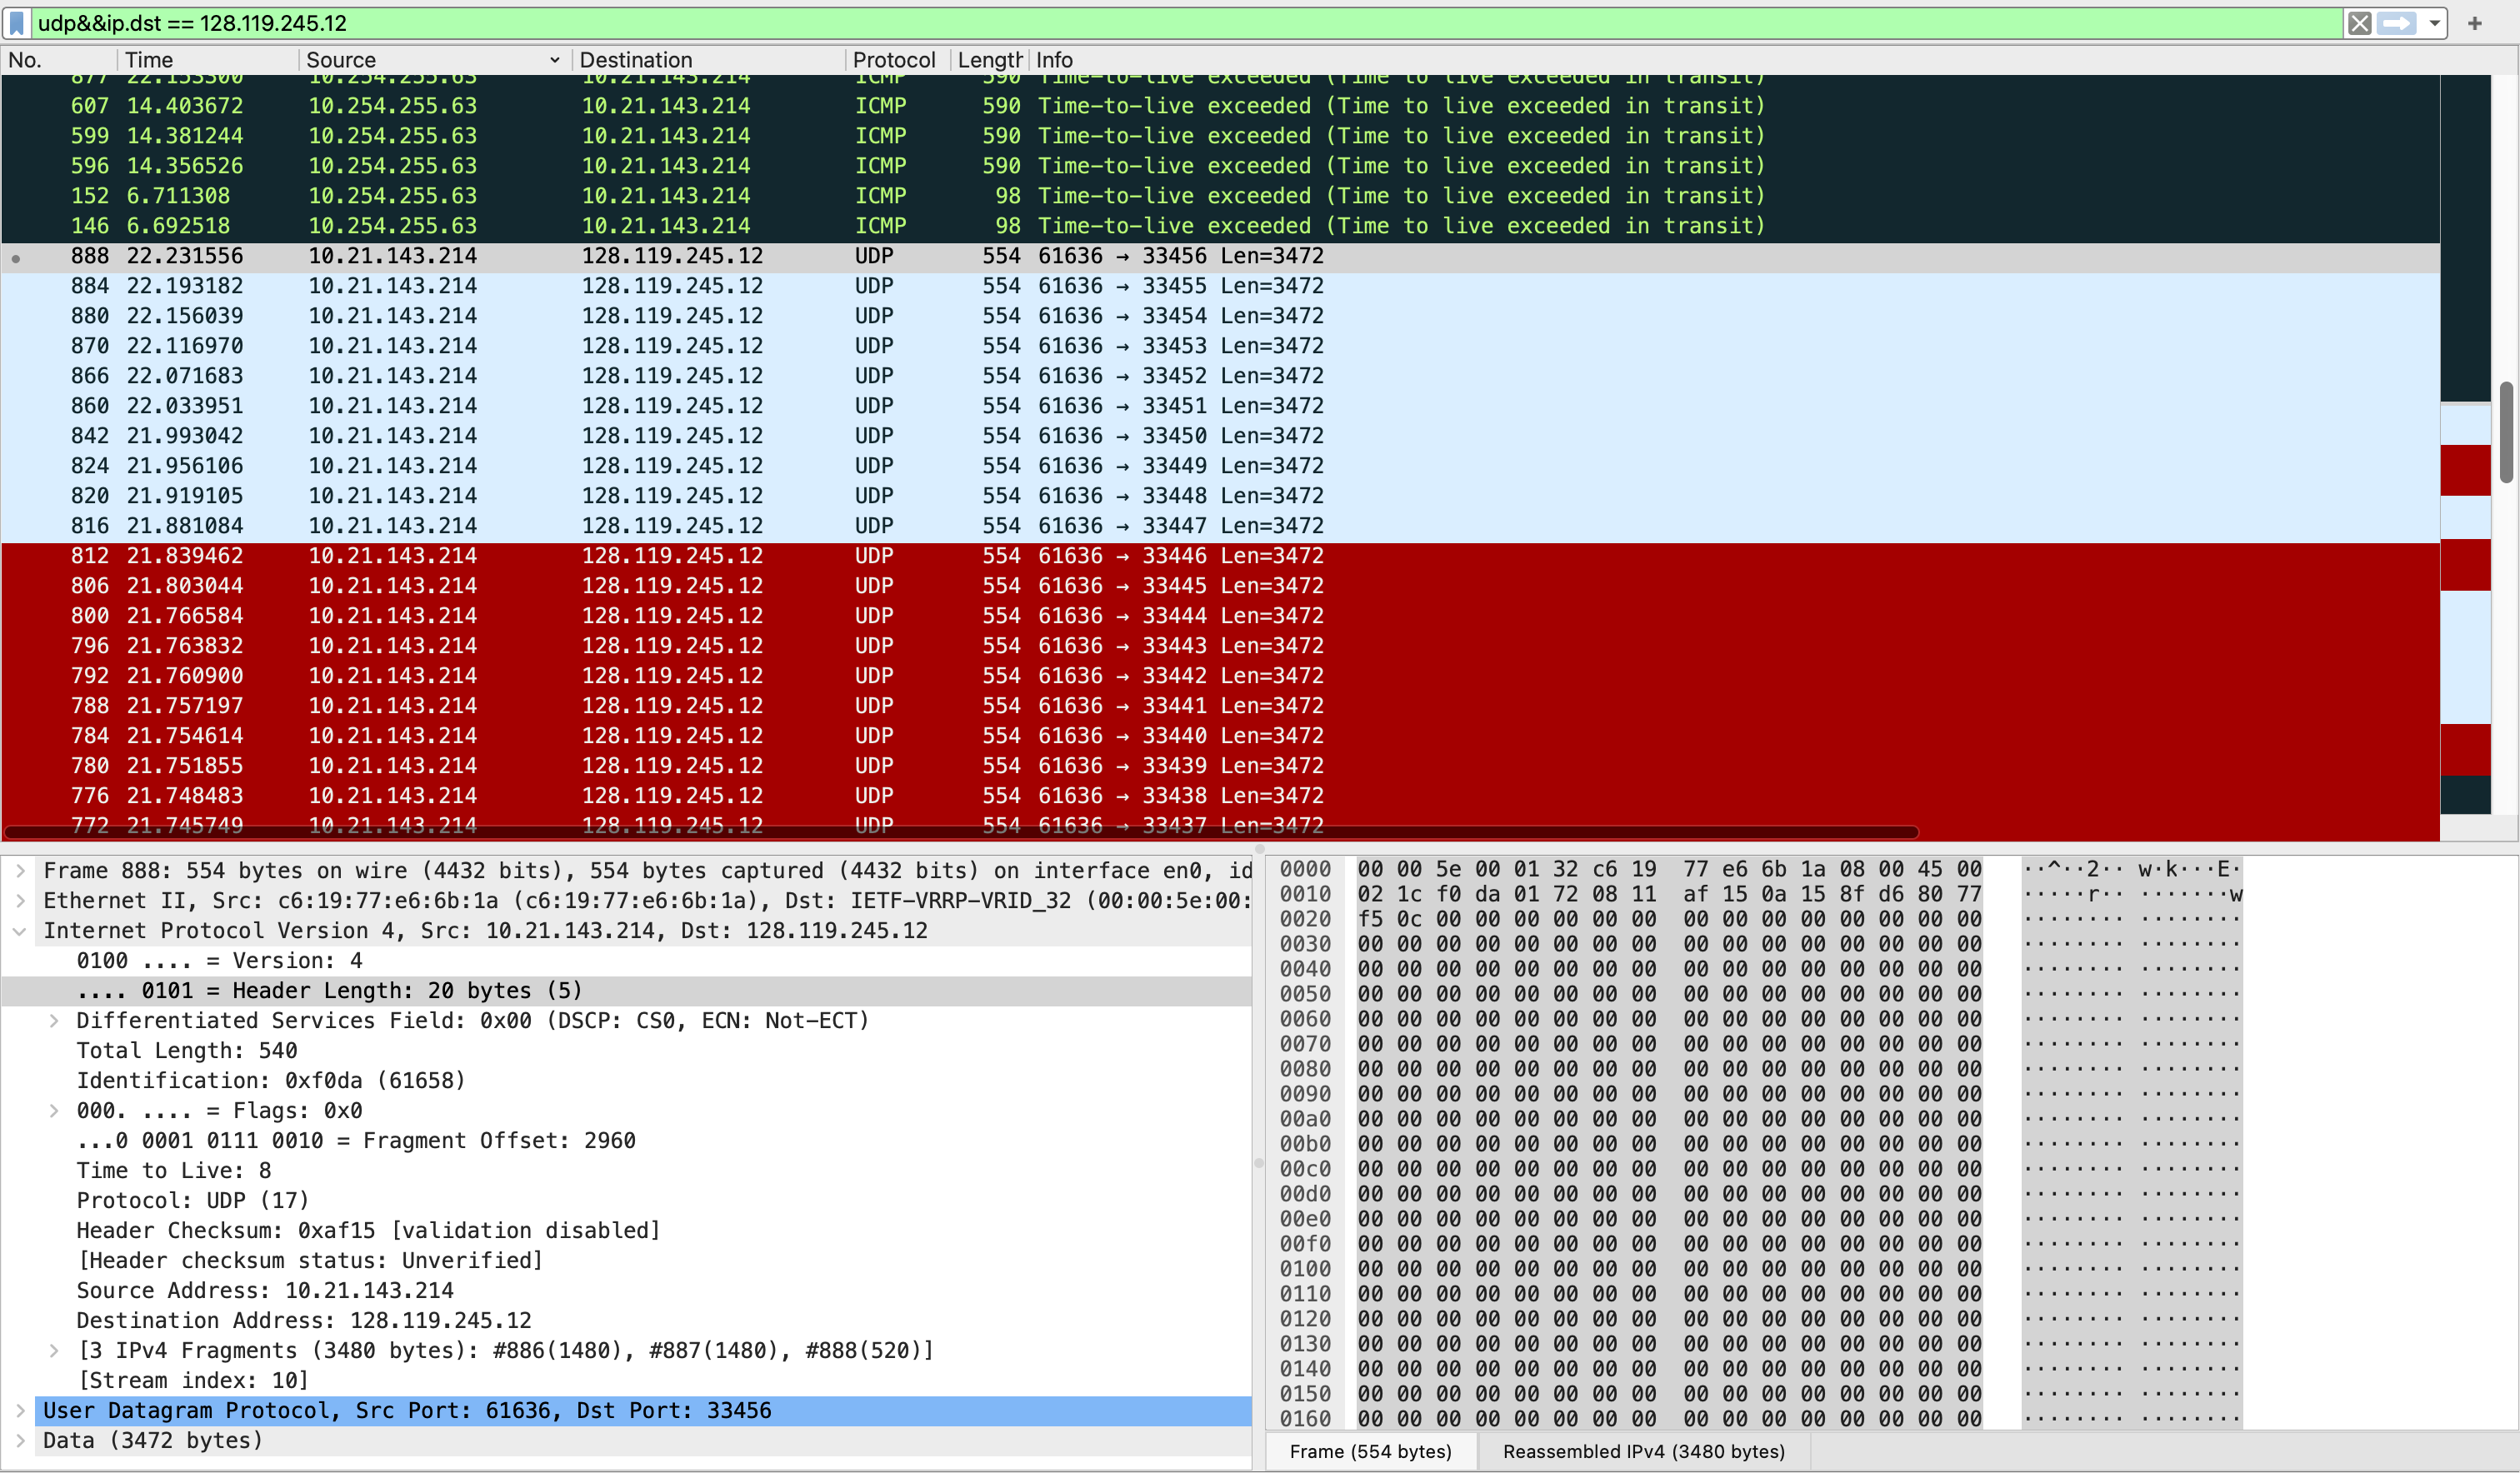
\includegraphics[width=1.0\textwidth]{5.png}
\end{figure}
\subsection{Question 5}
The always changing fields in the IP datagram are:
\begin{itemize}
    \item Identification: Different datagrams have different identification numbers.
    \item Header Checksum: It is changed as Identification changes.
\end{itemize}
\subsection{Question 6}
The constant fields in the IP datagram are:
\begin{itemize}
    \item Version: IPv4.
    \item Header Length: 20 bytes.
    \item Differentiated Services Field: 0x00 (DSCP: CS0, ECN: Not-ECT)
    \item Source Address and Destination Address.
    \item Protocol: UDP.
\end{itemize}
Identification and Checksum must be changing becuase each datagram is different and has the unique identification number, and the checksum is calculated based on the datagram with a changing identification number. Actually,
TTL is also changing for each traceout, but it is not included in the list because it is not always changing (maybe 2 or 3 datagrams have the same TTL). It might be caused by multiple datagrams packet capturing at the same time.
\\The Source and Destination Address must be constant, because I have made the filter with the fixed destination address while sorting with a fixed source address. The
protocol is also constant, because it is always UDP on MacOS. I suppose in the same traceout the version, total length, and fragment offset are also constant (the total length has changed but it is always 540, 520, or 56 bytes,
and I have made 3 traceouts at all).
\subsection{Question 7}
The Identification is always changing. Actually, the identification number is decreased by 1 for each datagram.
I think it is because now the time is in descending order, so actually when the datagram is captured in normal order (real-time), the identification number is increased by 1 for each datagram.
\section{ICMP TTLexceeded replies}
\begin{figure}[H]
    \centering
    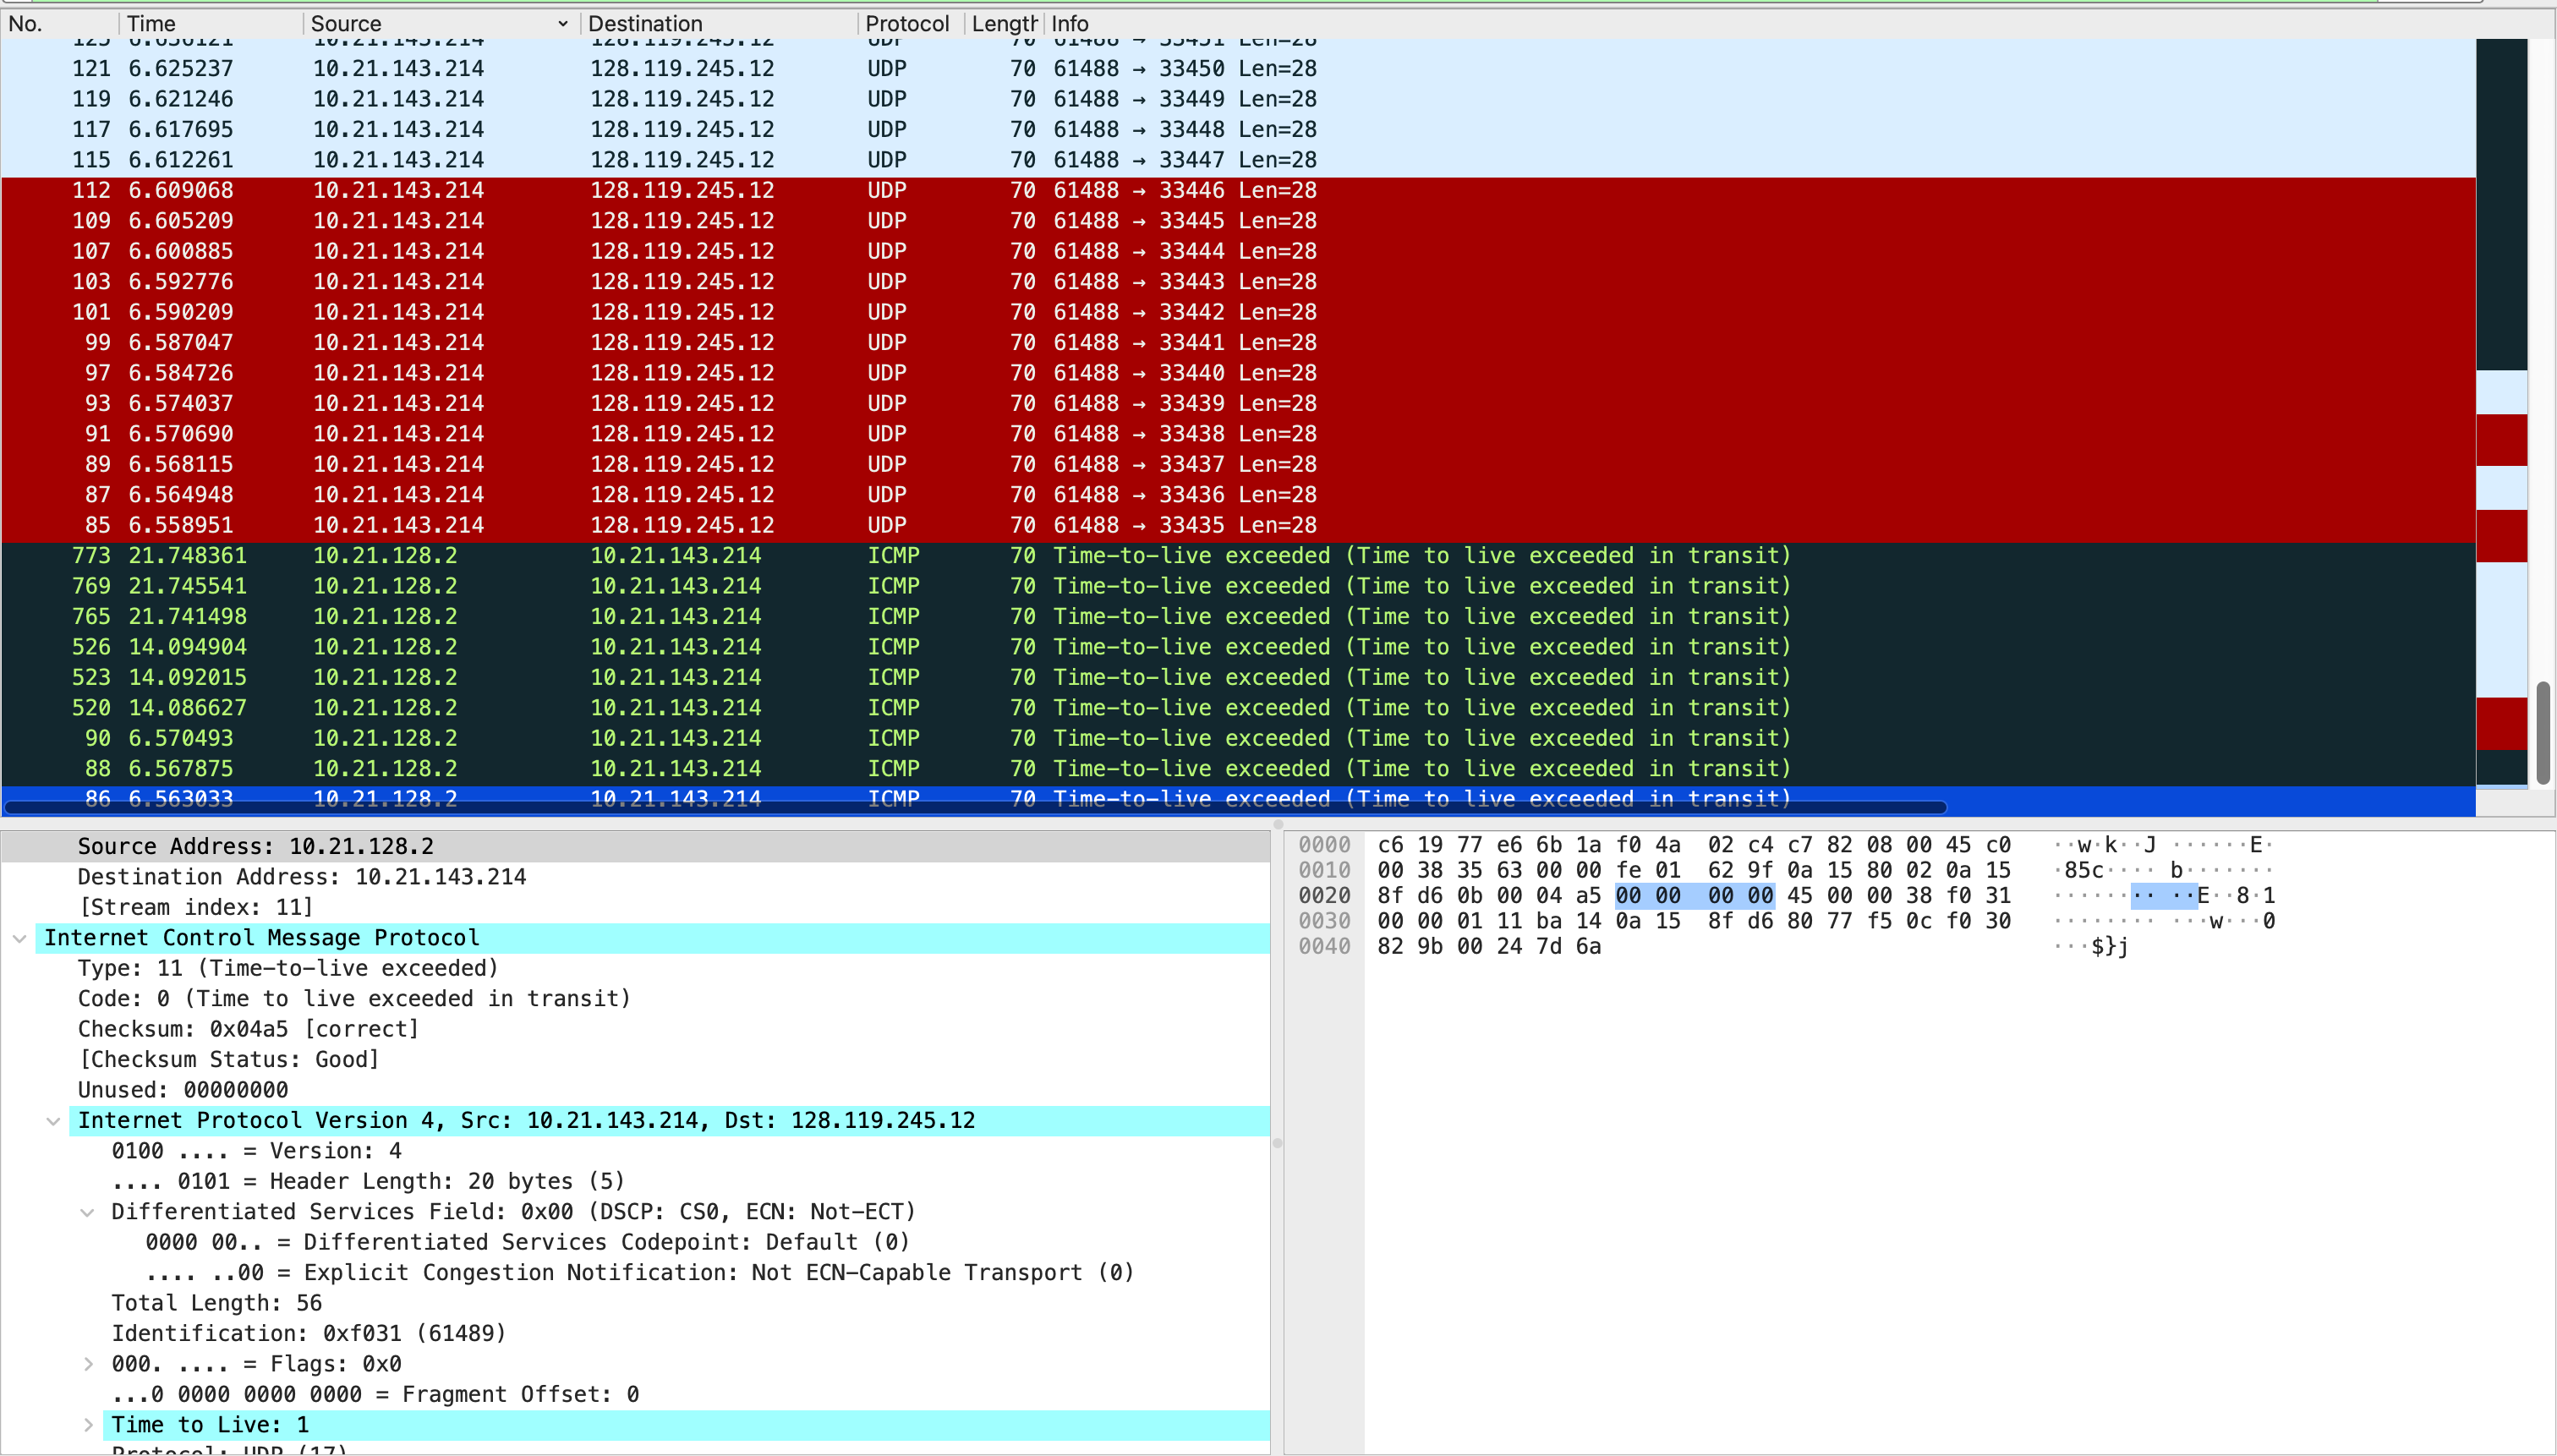
\includegraphics[width=1.0\textwidth]{8.png}
\end{figure}
The packet 773 - 86 shown in the figure above is the ICMP TTLexceeded reply by the first hop router. 
\subsection{Question 8-9}
More detailed information can be found in the attached file 8-9.pdf.
\begin{figure}[H]
    \centering
    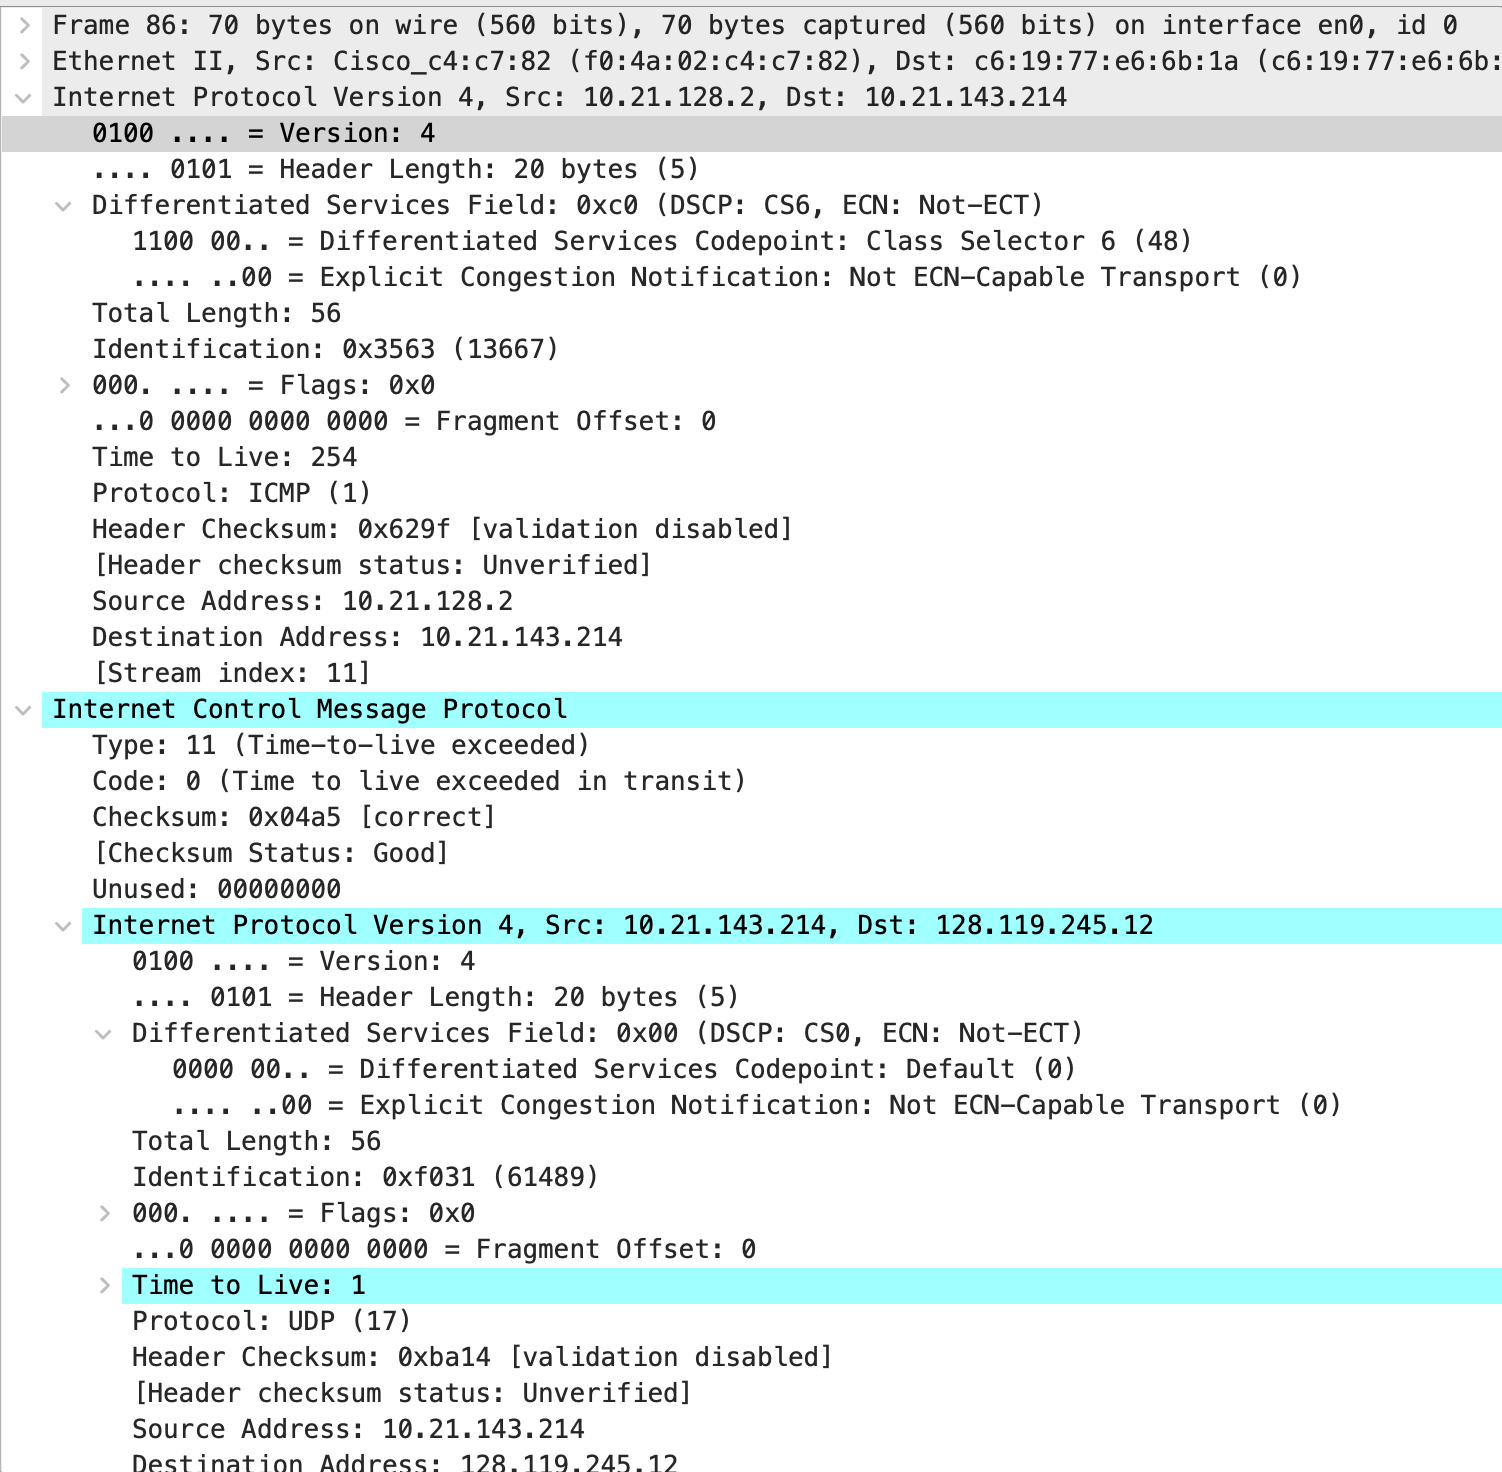
\includegraphics[width=1.0\textwidth]{9.png}
\end{figure}
In the IP protocol, the TTL field is always 254 which remains unchanged.
(But in the ICMP protocol, the TTL field is always 1.) The Identification field for frame 86 (screenshot above) is 0x3563 (13667).
This field is always changing.

\section{Fragmentation}
\begin{figure}[H]
    \centering
    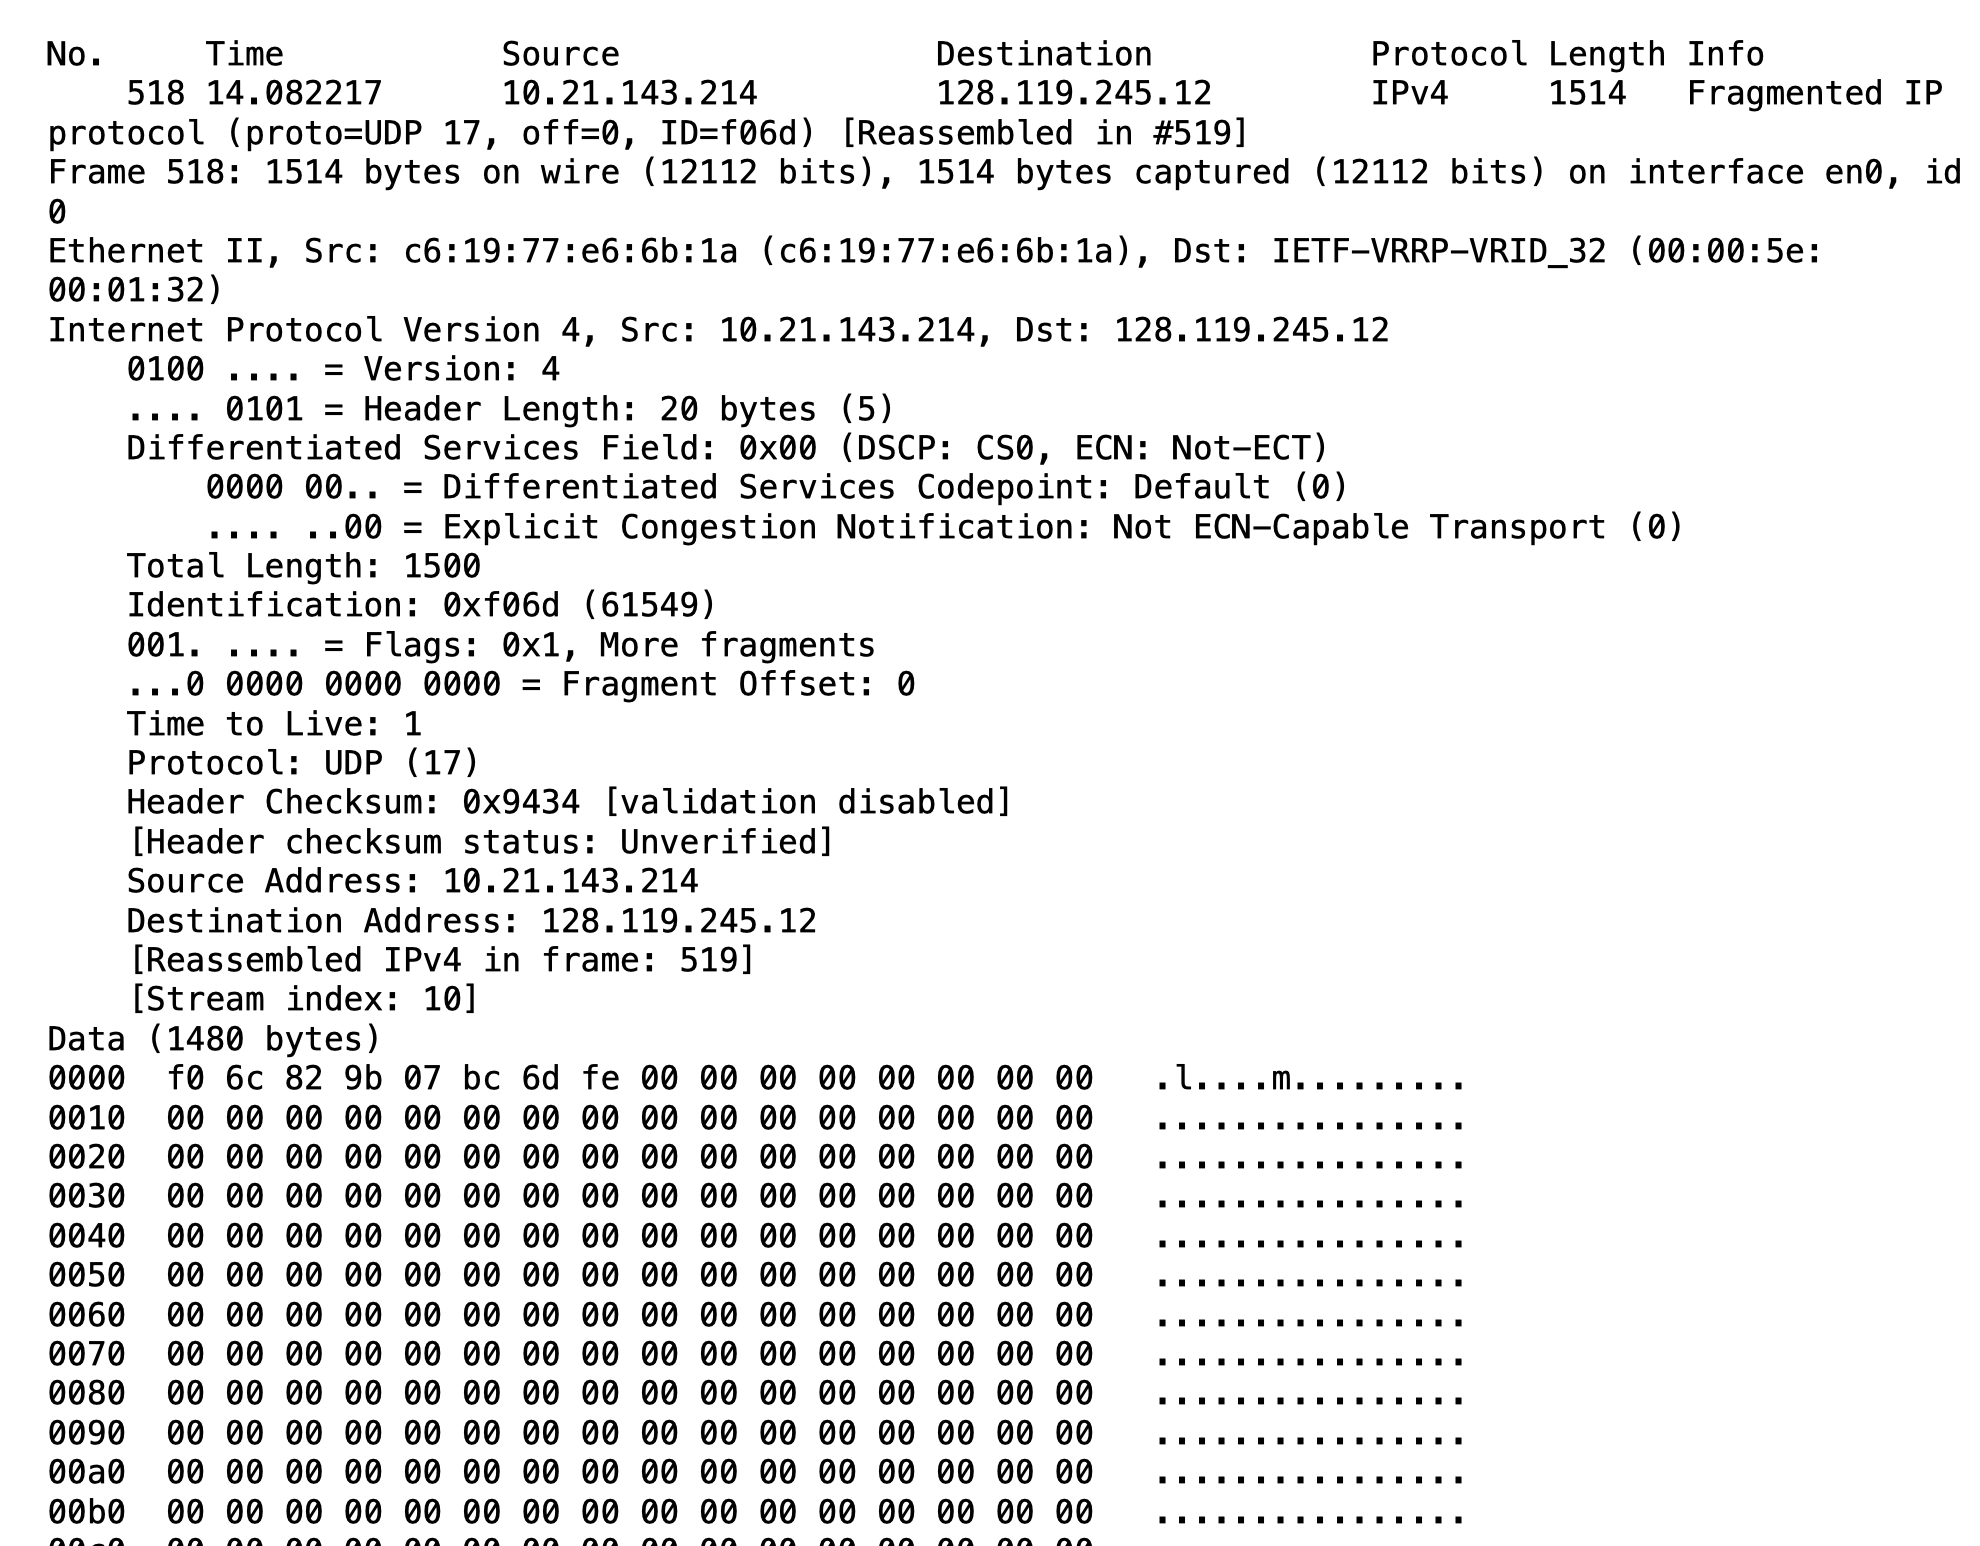
\includegraphics[width=1.0\textwidth]{10-1.png}
\end{figure}
\begin{figure}[H]
    \centering
    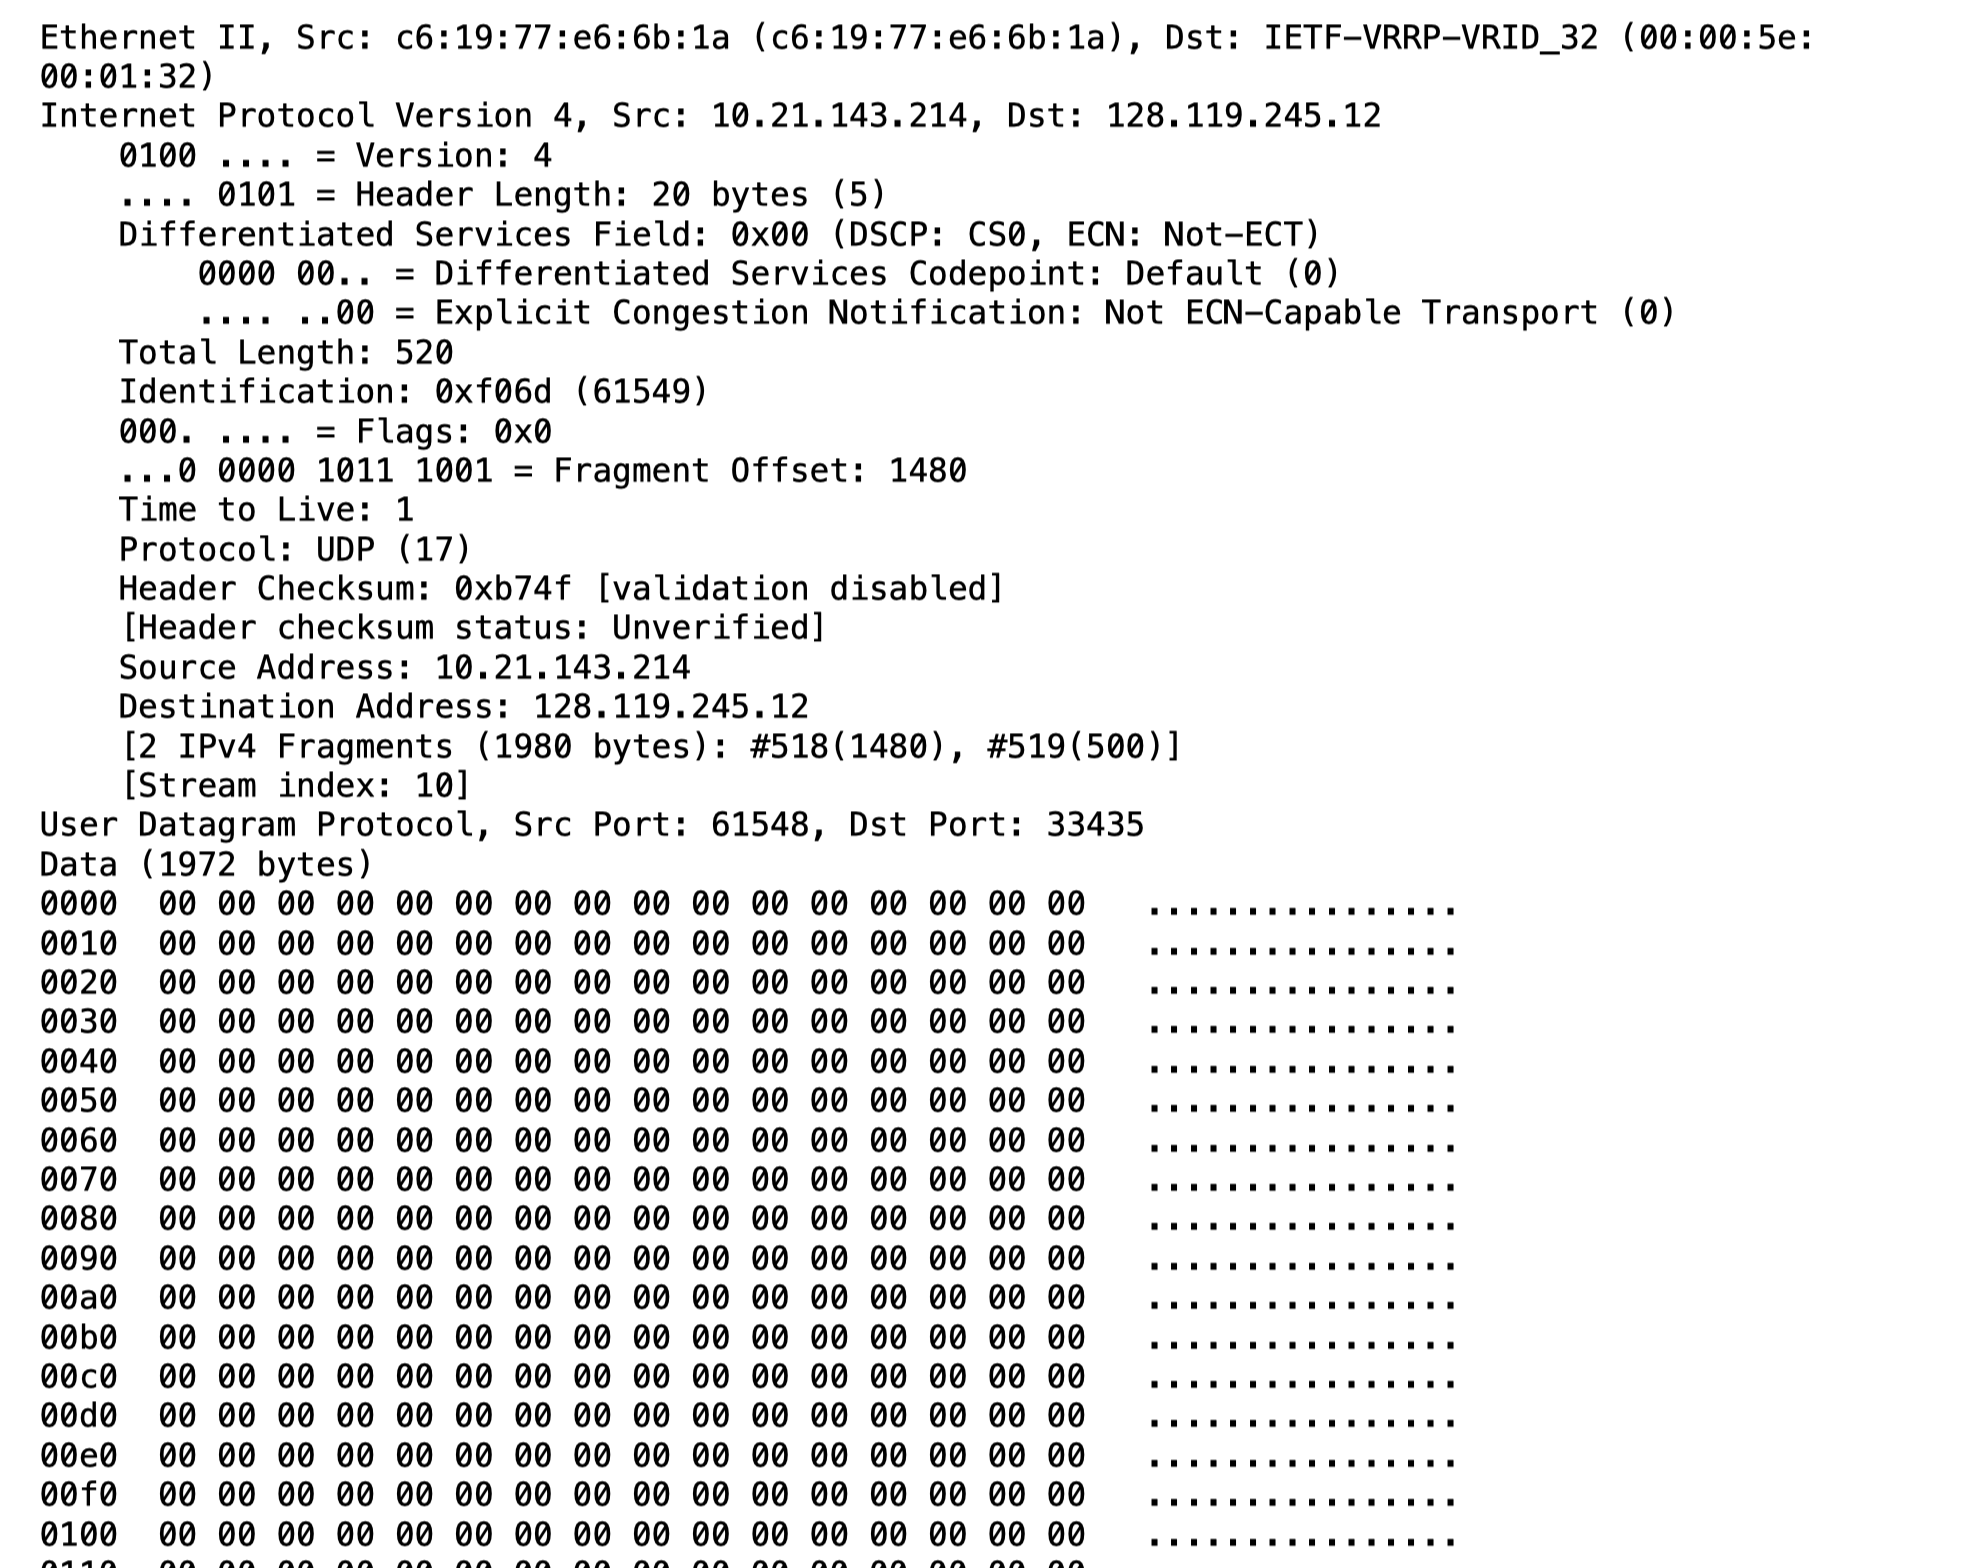
\includegraphics[width=1.0\textwidth]{10-2.png}
\end{figure}
The two figures above show the ICMP Echo Request message sent with a packet size of 2000 bytes. The first figure shows the first fragment, and the second figure shows the second fragment.
\subsection{Question 10-13}
Yes, the ICMP Echo Request message sent with a packet size of 2000 bytes has been fragmented into multiple IP datagrams.
\\It can be seen that the "Flags: 0x1" in the first fragment, and fragment offset is 0 which indicates that this is the first fragment (instead of a latter fragment).
This datagram length is 1500 bytes with the header length of 20 bytes and the payload length of 1480 bytes.
\\For the second fragment, fragment offset is 1480 which indicates that this is the second fragment (instead of a first fragment). There are no more
fragments after this datagram, so the "Flags: 0x0" indicates that this is the last fragment.
\\The changed fields are:
\begin{itemize}
    \item Identification: Different identification numbers for different fragments.
    \item Fragment Offset: 0 for the first fragment, 1480 for the second fragment.
    \item Flags: 0x1 for the first fragment, 0x0 for the second fragment.
    \item Total (and payload) Length: First fragment: 1500 bytes, second fragment: 520 bytes.
    \item Header Checksum: Changed as Identification changes.
\end{itemize}

\subsection{Question 14-15}
\begin{figure}[H]
    \centering
    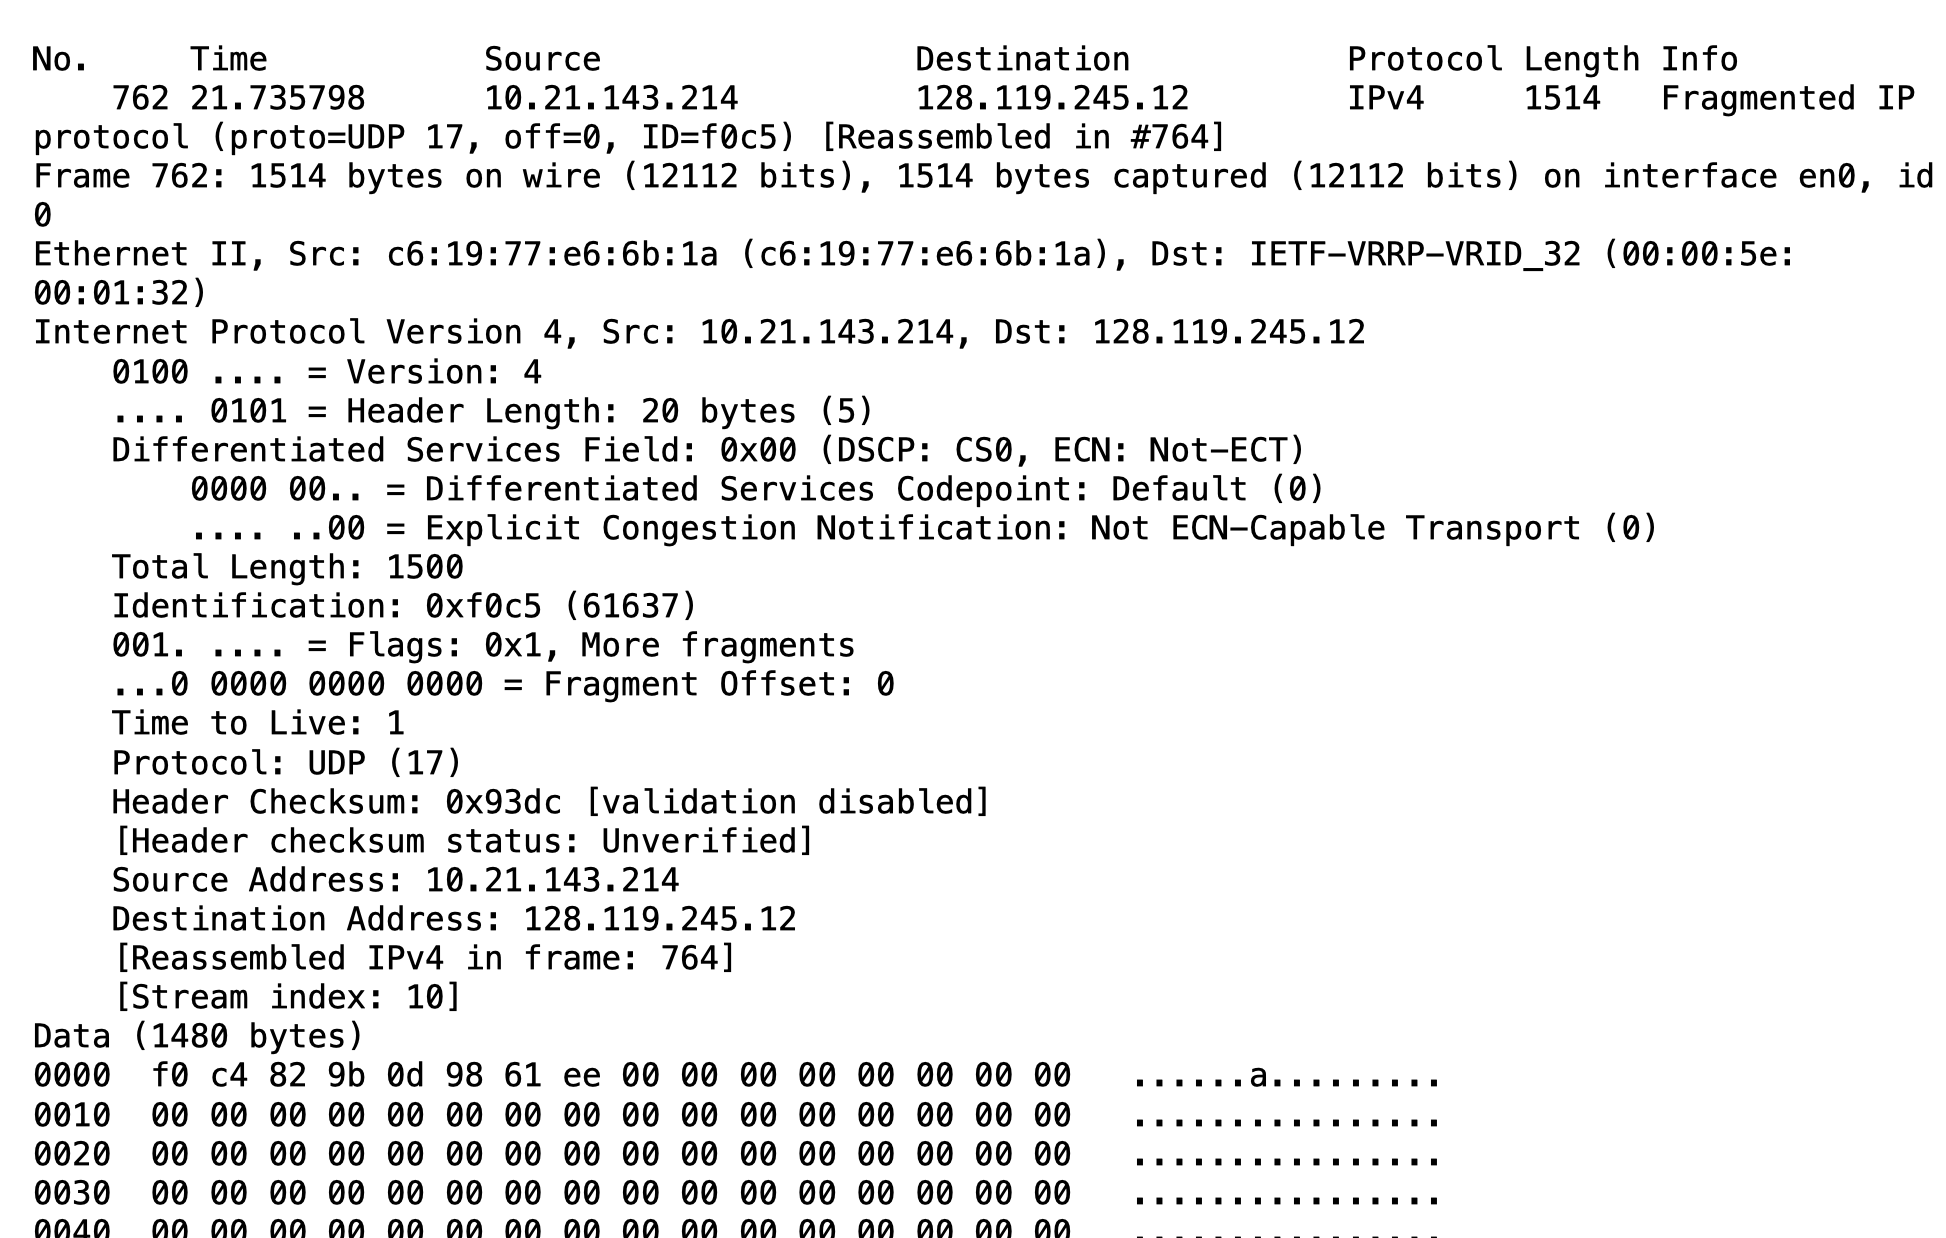
\includegraphics[width=1.0\textwidth]{14-1.png}
\end{figure}
\begin{figure}[H]
    \centering
    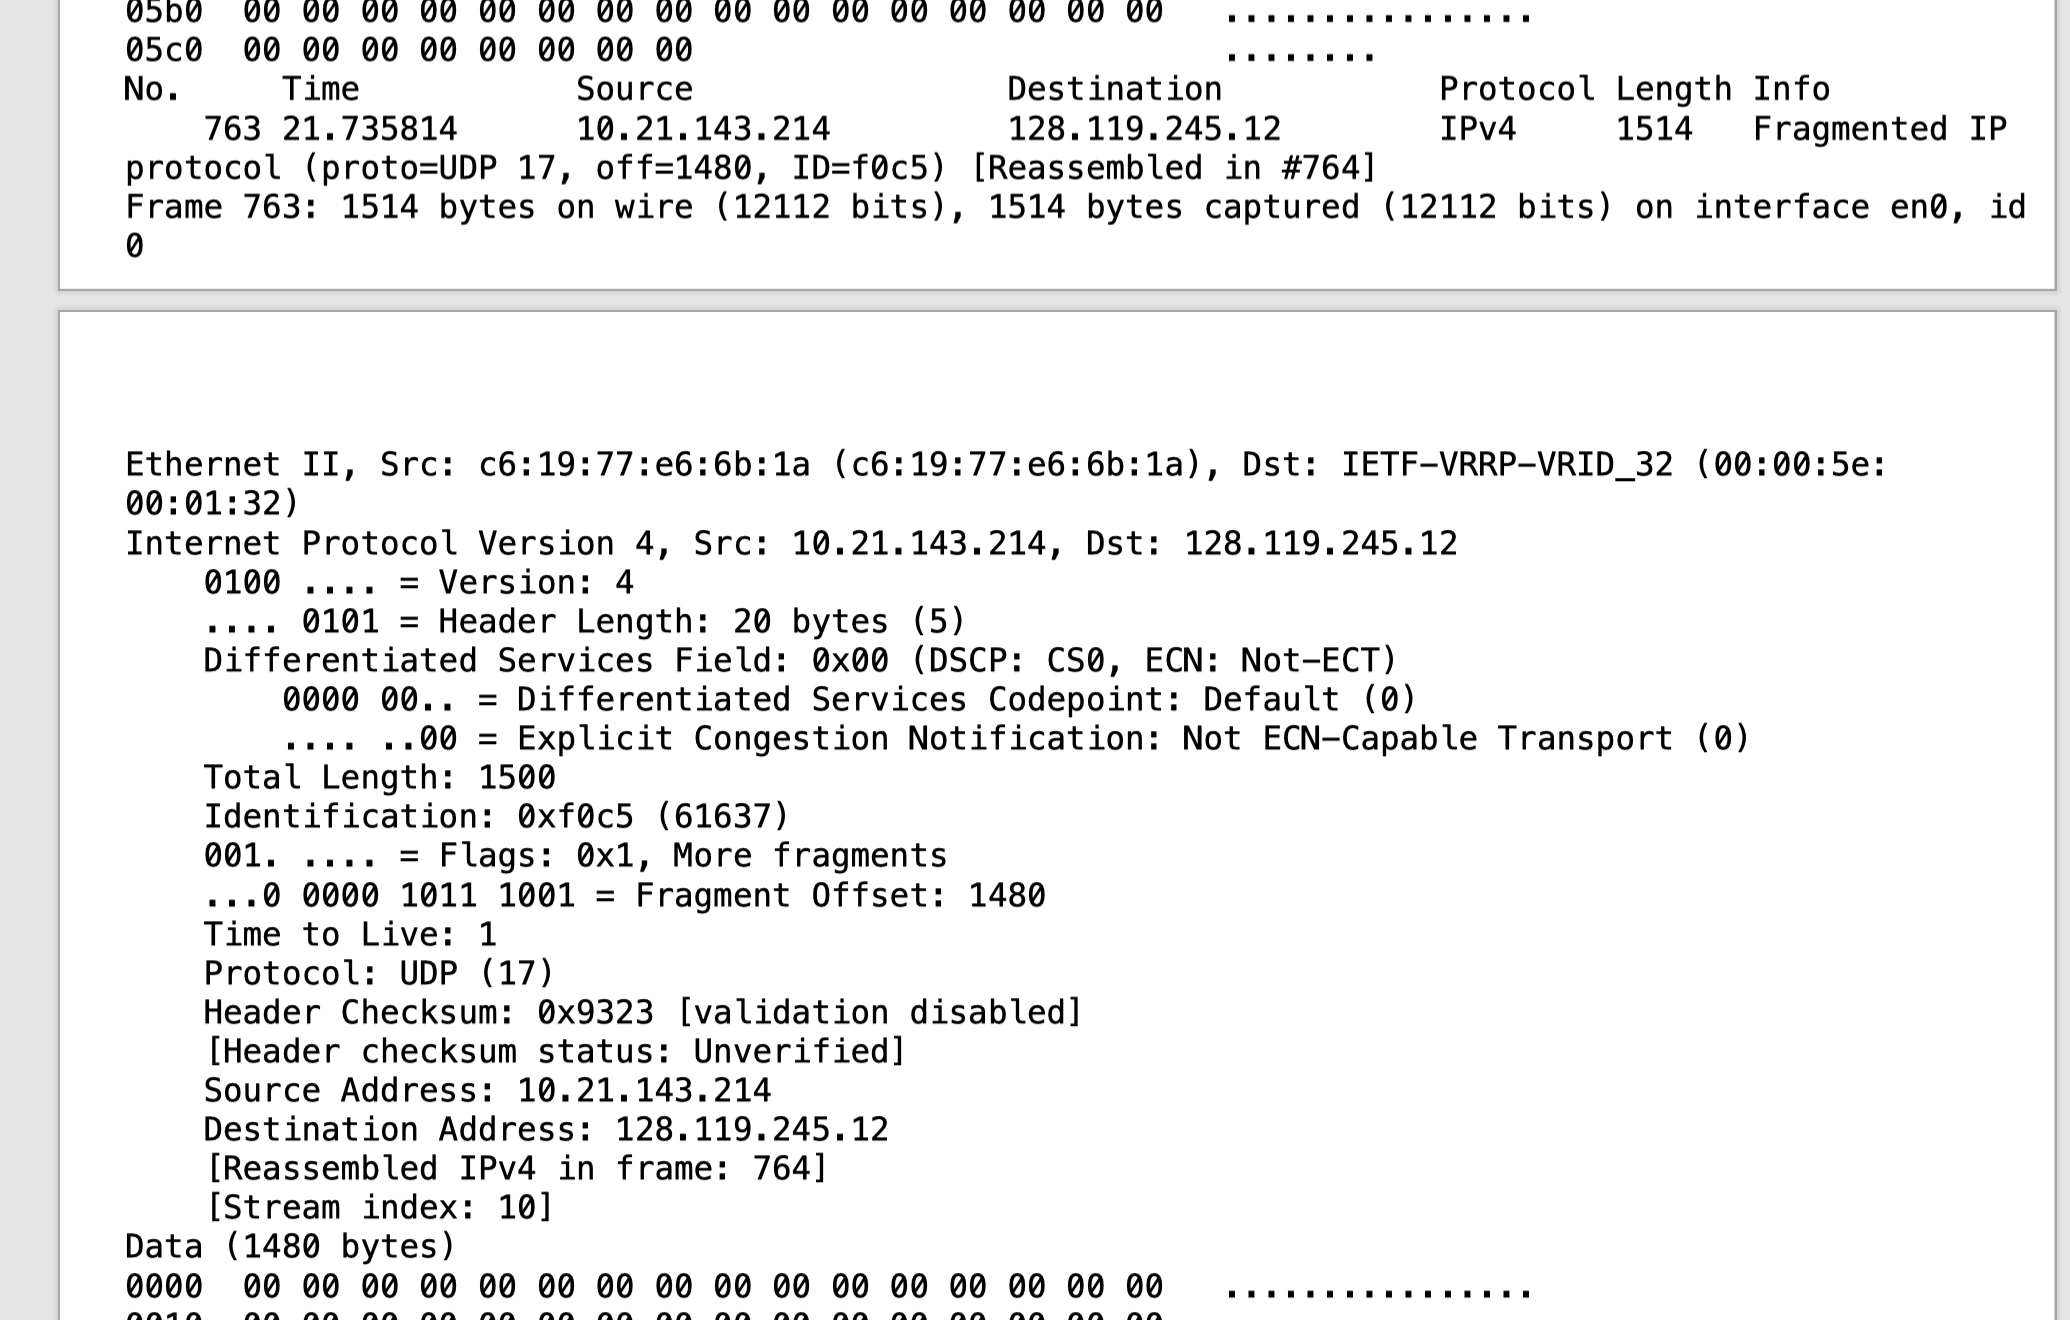
\includegraphics[width=1.0\textwidth]{14-2.png}
\end{figure}
\begin{figure}[H]
    \centering
    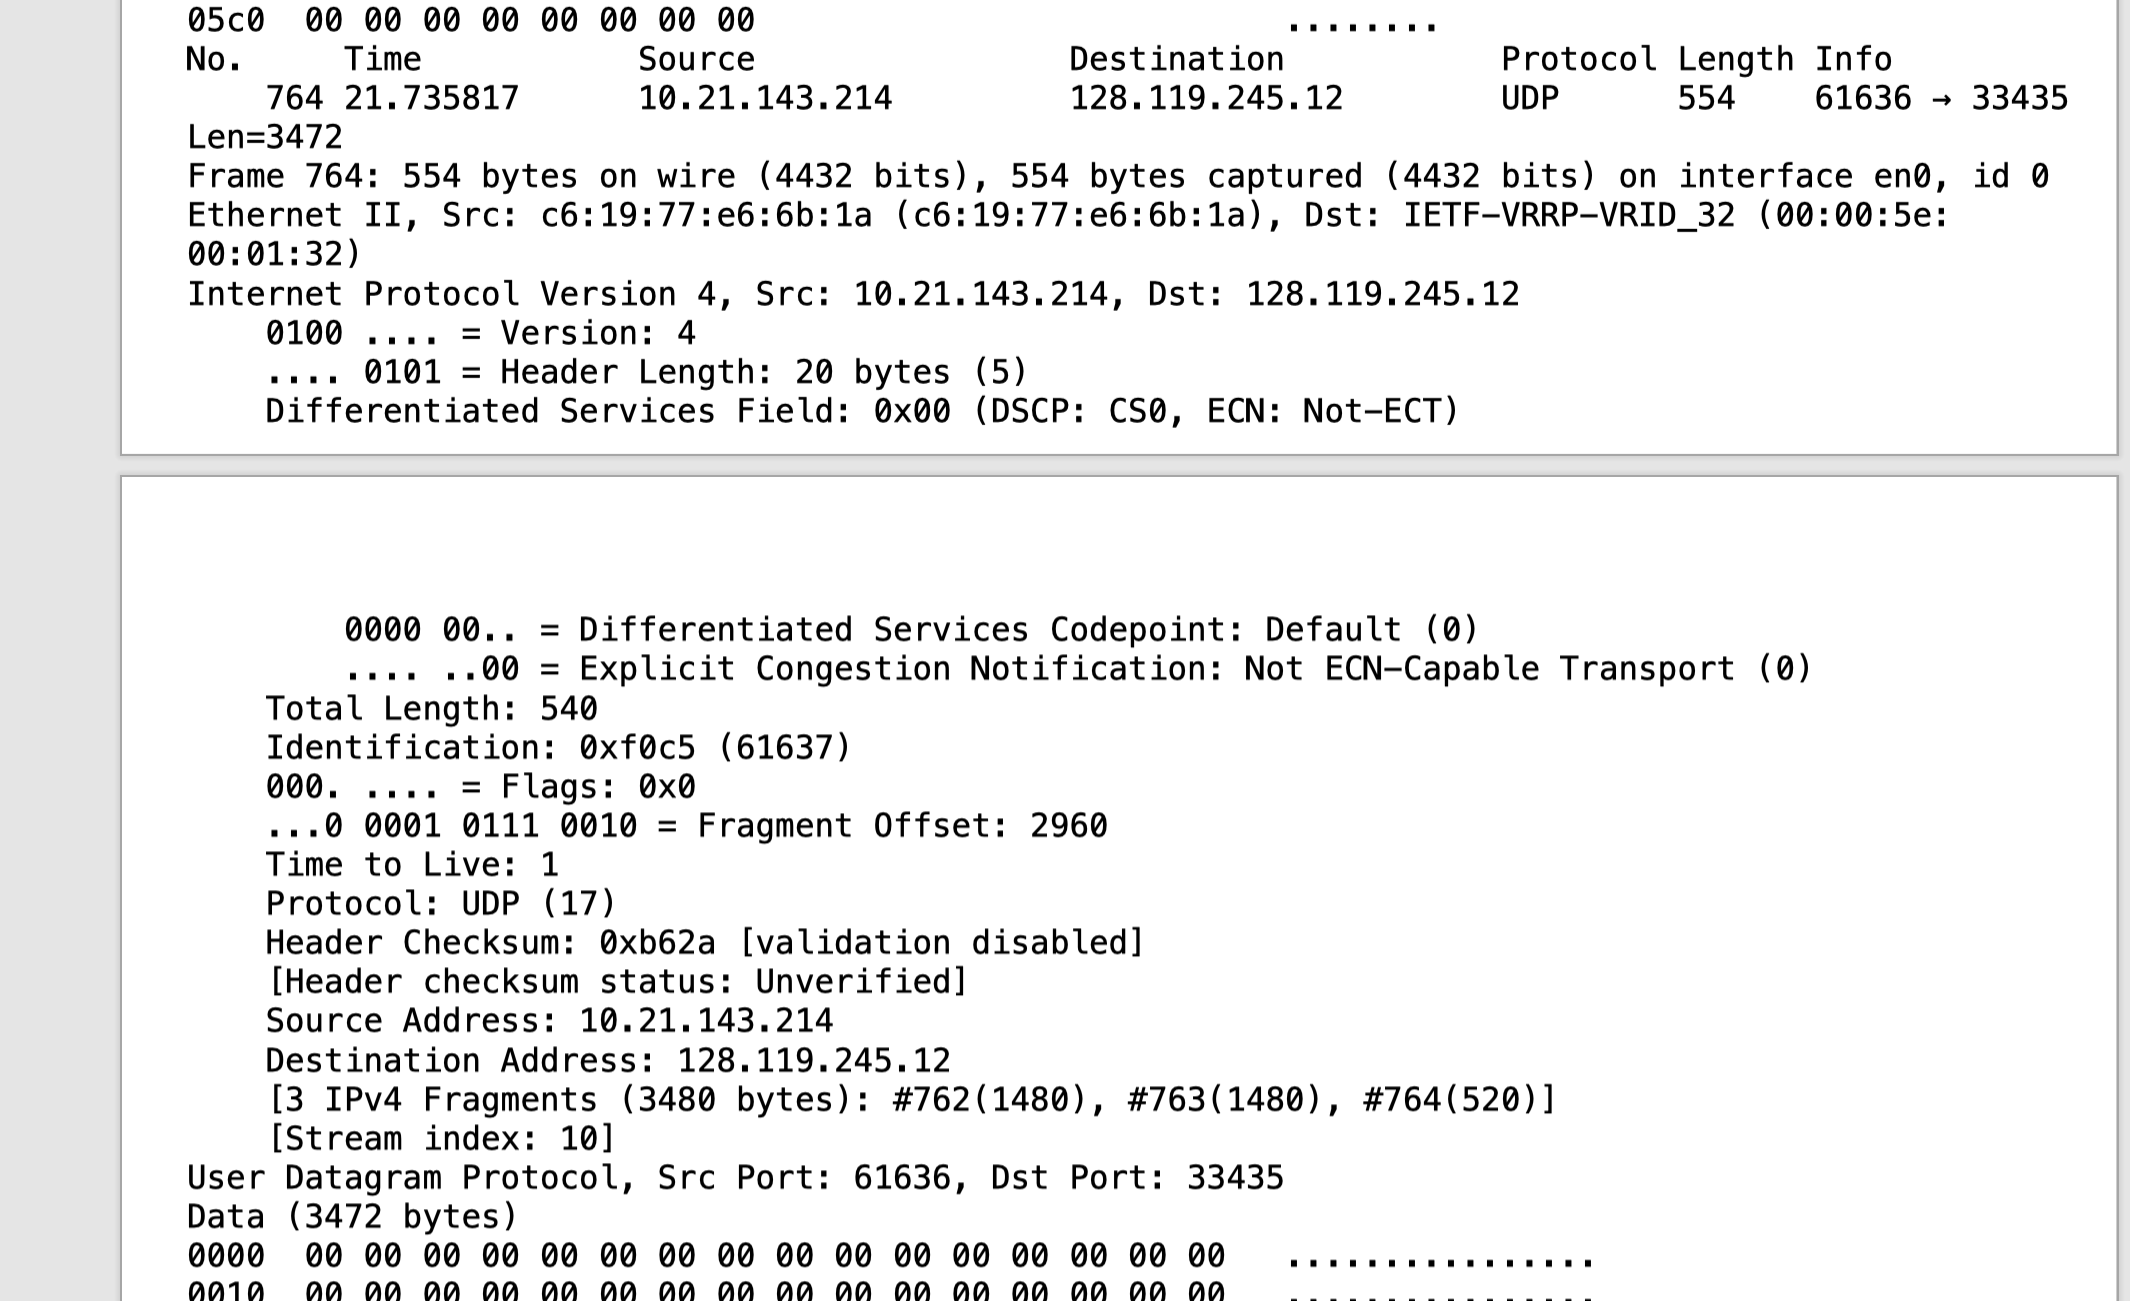
\includegraphics[width=1.0\textwidth]{14-3.png}
\end{figure}
The three figures above show the ICMP Echo Request message sent with a packet size of 3500 bytes.
So the total amount of fragments is 3:
The first fragment and the second fragment have "Flags: 0x1" and the third fragment has "Flags: 0x0".
Fields that are changed:
\begin{itemize}
    \item Identification: Different identification numbers for different fragments.
    \item Fragment Offset: 0 for the first fragment, 1480 for the second fragment, and 2960 for the third fragment.
    \item Flags: 0x1 for the first and second fragments, 0x0 for the third fragment.
    \item Total (and payload) Length: First fragment: 1500 bytes, second fragment: 1500 bytes, third fragment: 540 bytes.
    \item Header Checksum: Changed as Identification changes.
\end{itemize}
\end{CJK*}
\end{document}
